%% LyX 2.2.4 created this file.  For more info, see http://www.lyx.org/.
%% Do not edit unless you really know what you are doing.
\documentclass[12pt,italian]{book}
\usepackage[T1]{fontenc}
\usepackage[latin9]{inputenc}
\pagestyle{plain}
\setcounter{secnumdepth}{4}
\setcounter{tocdepth}{3}
\usepackage{babel}
\usepackage{verbatim}
\usepackage{float}
\usepackage{url}
\usepackage{graphicx}
\usepackage{setspace}
\onehalfspacing
\usepackage[unicode=true,
 bookmarks=true,bookmarksnumbered=false,bookmarksopen=true,bookmarksopenlevel=1,
 breaklinks=true,pdfborder={0 0 1},backref=false,colorlinks=false]
 {hyperref}
\hypersetup{pdftitle={Cloud Migration},
 pdfauthor={Andrea Decorte},
 pdfsubject={Cloud Computing},
 pdfkeywords={cloud, SCE, migration, enterprise, IBM}}

\makeatletter
%%%%%%%%%%%%%%%%%%%%%%%%%%%%%% Textclass specific LaTeX commands.
% Customized LaTeX preamble %%%%%%%%%%%%%%%%%%%%%%%%%%%

% --- Page geometry --- %
\usepackage{geometry}
\usepackage{url}
\geometry{
verbose,a4paper,lmargin=0.17\paperwidth,
rmargin=0.1\paperwidth
}

% Vertical length parameters

% Text height
\setlength\textheight{0.7\paperheight}
% Space at top of page
\setlength\topmargin{0pt}
% Space beteen header and text
\setlength\headsep{0.08\textheight}
% Space between text and footer (not footnote!)
\setlength\footskip{0.08\textheight}
% 2.5 lines space between text and footnote
\renewcommand\footnoterule{
\vspace{2.5em}
\kern-3\p@\hrule\@width.4\columnwidth%
\kern2.6\p@}
  
% --- Common packages --- %
\usepackage{amsmath,amsfonts,amssymb,amsthm,multicol}
\usepackage{epsfig,verbatim}
\usepackage{ifthen}

% --- Big letters at the beginning of chapters --- %
% "ptmri" is the italic version of "ptmr"
\newfont{\iniziocap}{ptmri scaled 5000}
\newcommand{\primalettera}[1]{
{\iniziocap #1}


\vspace*{-4em}\hangindent=4em\hangafter=-3\hspace*{-1.5em}}

% --- Fonts --- %
%\usepackage{ae}
%\usepackage{aecompl}
%\usepackage{lmodern}
\renewcommand{\rmdefault}{ptm}
\renewcommand{\sfdefault}{phv}
\renewcommand{\ttdefault}{pcr}
\renewcommand{\sldefault}{it}


% --- For clickable URL's --- %
\usepackage{hyperref}

% --- Fancy headers --- %
\usepackage{fancyhdr}

% --- Useful commands --- %
\newcommand{\clearemptydoublepage}{
\newpage{\pagestyle{empty}
\cleardoublepage}
}

% --- Andrea: Add unnumbered chapters to index and fix the headers --- %
\newcommand{\aggiungiAIndice}[1]
{ %adds chapter to index with the chosen name
\addcontentsline{toc}{chapter}{\protect\numberline{}#1}
%adds the correct header check fancyhdr docs
\markboth{#1}{} 
}

\newcommand{\@titolo}{?}

\newcommand{\@facolta}{?}

\newcommand{\@corso}{?}

\newcommand{\@annoaccademico}{?}

\newcommand{\@sessione}{i}

\newcommand{\@relatore}{?}

\newcommand{\@laureando}{?}

\newcommand{\facolta}[1]{
 \renewcommand{\@facolta}{
 \uppercase{facolt\`a di #1}}}

\newcommand{\corso}[1]{
 \renewcommand{\@corso}{\uppercase{#1}}}

\newcommand{\annoaccademico}[1]{
 \renewcommand{\@annoaccademico}{#1}}

\newcommand{\sessione}[1]{
 \renewcommand{\@sessione}{\uppercase{#1}}}

\newcommand{\relatore}[2][Chiar.mo Prof. Ing.]{
 \renewcommand{\@relatore}{#1\\ \uppercase{#2}}}

\newcommand{\laureando}[1]{
 \renewcommand{\@laureando}{\uppercase{#1}}}

\newcommand{\titolo}[1]{
 \renewcommand{\@titolo}{\uppercase{#1}}}

% --- Personalized title page --- %
\renewcommand{\maketitle}{
 \begin{titlepage}{
  \vspace*{-0.1\textheight}
  \begin{center}\begin{large}
   \uppercase{alma mater studiorum -- universit\`a di bologna\\}
   \medskip\end{large}
   \smallskip
   \rule{\textwidth}{.4pt}\\
   \vfill 
   \begin{large}
   \uppercase{\@facolta\\}
   \vfill
   \ifthenelse{\not\isundefined{\@corsodilaureaspec}}
   {\uppercase{corso di laurea specialistica in \@corsodilaureaspec\\}}
   {\ifthenelse{\not\isundefined{\@corsodilaurea}}
   {\uppercase{corso di laurea in \@corsodilaurea\\}}{}}\end{large}

   \begin{large}
    \ifthenelse{\isundefined{\@correlatorea}}{\vspace{16ex}}
    {\ifthenelse{\isundefined{\@correlatoreb}}{\vspace{10ex}}{\vspace{6ex}}}

    {\setlength{\baselineskip}{1.5\baselineskip}

     \begin{huge}\@titolo\end{huge}\\}

    \ifthenelse{\isundefined{\@correlatorea}}{\vspace{16ex}}
    {\ifthenelse{\isundefined{\@correlatoreb}}{\vspace{10ex}}{\vspace{6ex}}}

    Tesi in\\
    \@corso\\
    \vfill        
    \begin{multicols}{2}
     \raggedright
     \emph{Relatore}:\\
     \@relatore\\
  
     \ifthenelse{\isundefined{\@correlatorea}}{}{
      \bigskip
      \emph{Correlatore}:\\
      \vfill
      \@correlatorea\\
     }

     \ifthenelse{\isundefined{\@correlatoreb}}{}{
      \bigskip
      \emph{Correlatore}:\\
      \vfill
      \@correlatoreb\\
     }

     \columnbreak
     \raggedleft
     \emph{Presentata da}:\\
     \@laureando\\	  

    \end{multicols}

    \vfill
    \rule{\textwidth}{.4pt}\\
    \vfill
    Sessione \@sessione\\
    \vfill
    Anno Accademico \@annoaccademico\\
    \end{large}\end{center}	
}\end{titlepage}}

% --- Dedication command --- %
\newcommand{\dedica}[1]{
  \clearemptydoublepage
  \thispagestyle{empty}
  \vspace*{10ex}
  \begin{Large}
    \begin{flushright}
      \emph{#1}
    \end{flushright}
  \end{Large}
  \vfill
  \clearemptydoublepage
}
%%%%%%%%%%%%%%%%%%%%%%%%%%%%%%%%%%%%%%%%%%%%%%%%%%%%%%%
\newcommand{\@corsodilaurea}{?}
\newcommand{\corsodilaurea}[1]{
  \renewcommand{\@corsodilaurea}{\uppercase{#1}}}

\makeatother

\usepackage{listings}
\renewcommand{\lstlistingname}{Listato}

\begin{document}

\facolta{Ingegneria}

\corsodilaurea{Ingegneria dell'Automazione}

\titolo{Analisi di soluzioni di motion control per azionamenti BLDC nel progetto
AlmaX}

\corso{Ingegneria dei Sistemi di Controllo}

\laureando{Filippo Guarda}

\relatore{Andrea Tilli}

\sessione{iii}

\annoaccademico{2019-2020}
\maketitle

\dedica{To everybody}

\begin{frontmatter}

\tableofcontents{}

\listoffigures

\end{frontmatter}

\begin{mainmatter}

% Questi abbelliscono l'intestazione delle pagine
% successive a quella di inizio capitolo.
\pagestyle{fancy}

% Nomi dei capitoli in lowercase nelle intestazioni
\renewcommand{\chaptermark}[1]{
 \markboth{\MakeUppercase{
 \chaptername}\ \thechapter.
 \ #1}{}}

\fancyhead[EL,OR]{\leftmark}
\fancyhead[OL,EC,OC,ER]{ }

\chapter*{Introduzione\aggiungiAIndice{Introduzione}}

\primalettera{L}a ERC, European Rover Challenge, � una competizione
a livello europeo organizzata dal 2014 in Polonia. Anche l'universit�
di Bologna, in collaborazione con la sede di Forl�, partecipa a questa
competizione con il gruppo AlmaX, che ha il compito di sviluppare
un rover che rispetti le specifiche fornite nel regolamento \cite{rules},
tra cui: 
\begin{itemize}
\item Un peso pari o inferiore a 50kg.
\item La capacit� di movimento autonomo attraverso computer vision e mapping
topografico, oltre alla possibilit� di inviare comandi al rover da
una base station via link radio.
\item La capacit� del rover di attraversare ostacoli e terreno accidentato
simile al suolo marziano.
\item La capacit� del rover di interagire con un pannello di controllo fisico
\end{itemize}
L'argomento di questa tesi � il benchmark del motion control del Rover. 

\section{Pipeline}

I motori BLDC forniti sono Siboni ProPlanet S60 ed S40 dotati di freno
integrato ed encoder incrementale, ognuno controllato da un drive
MicroPhase MicroOne, che riceve in broadcast istruzioni attraverso
un seriale CAN. Le istruzioni sono codificate in CANopen da un adattatore
Peak Usb collegato a un computer di bordo su cui � installato ROS
(Robot Operative System), il quale a sua volta riceve messaggi da
una base station sulla quale � sempre installato ROS.

\begin{comment}
TODO inserire immagine
\end{comment}
.

Nel capitolo 1 si studieranno nello specifico l'hardware e i metodi
utilizzati per connettere i diversi elementi del progetto, nel capitolo
2 si studier� il software necessario a permettere la comunicazione
tra i componenti. Nel capitolo 3 si elencheranno le problematiche
incontrate. 

\chapter{Architettura e componenti Hardware}

\section{Motori BLDC }

\primalettera{O}bbiettivo del progetto � il controllo di un motore
BLDC, in questo caso i motori forniti sono Siboni S60 ed S40. Questi
motori hanno le seguenti specifiche, che ci saranno utili pi� tardi
per inserirle nei parametri del drive: 

\begin{comment}
INSERIRE TABELLA
\end{comment}

I motori dispongono di connettori di tipo %
\begin{comment}
INSERIRE TIPOLOGIA CONNETTORI
\end{comment}
, con la seguente schematica: 

\begin{comment}
INSERIRE IMMAGINE
\end{comment}


\section{Computer di bordo}

Nel rover, il computer di bordo � una UPboard, molto comoda in quanto
estremamente modulare e dotata di moduli extra. Tra i muduli disponibili
� presente anche uno dotato di porte seriali CAN e rs422, molto utile
ai fini del progetto in quanto riduce il numero di connettori extra. 

Per questo progetto, non essendo disponibile la UPboard � stato utilizzato
un normale computer che utilizza linux come OS.

\section{Drive}

Il drive che guida il motore in PWM � un Microphase MicroOne, con
le seguenti specifiche: 

\begin{comment}
INSERIRE TABELLA
\end{comment}

Il drive � collegato al motore attraverso due connettori. Uno di potenza,
attraverso cui passano le fasi della PWM, il ground e la linea che
disattiva il freno integrato nel motore. L'altro responsabile della
ricezione del feedback di posizione da parte dell'encoder incrementale
e dei sensori di Hall. 

Sul drive sono anche presenti due attacchi RJ45 che il drive usa per
comunicare attraverso connessione seriale. 

\section{Convertitore Moxa e adattatore PCAN}

Per connettere il drive ai due computer utilizzati, uno per la programmazione
dello stesso e uno per il controllo, si usano due connettori da usb
a seriale

\subsection{MOXA}

Per programmare parametri e registri del drive � necessario utilizzare
un software proprietario (di cui si parler� nel dettaglio nel capitolo
2) che comunica attraverso una connessione seriale rs 422 resa possibile
da un convertitore moxa

\begin{comment}
INSERIRE IMMAGINE
\end{comment}


\subsection{PCAN}

Invece la comunicazione con il computer di bordo avviene su bus CAN,
attraverso l' adattatore PCAN.

\begin{comment}
INSERIRE IMMAGINE E BIBLIOGRAFIA
\end{comment}

L' adattatore � dotato di un led che ne comunica lo stato: 
\begin{itemize}
\item LED acceso: usb connessa al computer, nessuna comunicazione
\item LED lampeggia lentamente: adattatore attivo
\item LED lampeggia velocemente: trasmissione in corso
\end{itemize}

\section{Adattatori}

Sia il convertitore moxa che il PCAN utilizzano per la connessione
seriale degli attacchi DB9, di cui solo una parte dei pin � effettivamente
utilizzata. Questo � un problema in quanto il drive dispone solo di
attacchi rj45. Per ovviare al problema sono stati cablati a mano due
adattatori. 

\subsection{Adattatore per MOXA}

Bench� dalla documentazione del convertitore moxa non venga specificato
su quali pin passi la linea seriale rs422, nella confezione � fornito
un attacco extra che presenta connessioni ben definite. Utilizzando
la schematica degli attacchi RJ45 fornita nel datasheet del drive
� stato cablato a mano un cavo ethernet con un RJ45 da un lato e cavi
scoperti dall'altro, in modo da poterli connettere con l'attacco fornito.

\begin{comment}
INSERIRE IMMAGINE E BIBLIOGRAFIA
\end{comment}


\subsection{Adattatore per PCAN}

Anche l' adattatore Peak dispone di un attacco db9, di cui solo 4
pin vengono utilizzati. Il bus can passa attraverso i pin 2 (Can H)
e 7 (Can L) %
\begin{comment}
controllare pin effettivi
\end{comment}
questi due pin devono essere collegati ai pin n. 2 e 3 dell'attacco
rj45. Questa connessione si effettua tramite un adattatore cablabile
di facile reperibilit�. Quello utilizzato in questo progetto nello
specifivo � stato acquistato su amazon (link prodotto) ed ha i pin
dell'attacco rj45 femmina codificati tramite i colori dei cavetti
che vanno inseriti manualmente nell'attacco db9 femmina, secondo questa
schematica: 

\begin{comment}
INSERIRE IMMAGINE E BIBLIOGRAFIA
\end{comment}


\section{Alimentatori}

Per il progetto servono due alimentatori separati, uno di potenza
(BK precision 9104), che alimenta il controllo PWM a 48V (nel rover
l'alimentazione sar� fornita da una batteria a 48V) e uno riservato
alla parte logica, che alimenta il drive a 24V.


\chapter{Introduzione a ROS, CAN e CANopen.}

\primalettera{I}l modello di motion control � basato su ROS, che
facilita la comunicazione tra diverse macchine su cui � installato,
nel nostro caso tra la base station e il computer di bordo attraverso
un link radio. 

Uno dei pregi di ROS � la possibilit� di installare librerie aggiuntive
che lo dotano di funzionalit� extra, tra le quali la possibilit� di
codificare istruzioni in CANopen. Queste istruzioni servono a controllare
il drive, passando attraverso il datalink layer CAN.

In questo capitolo si parler� nello specifico di ROS, CANopen over
CAN.

\section{ROS}

ROS, o Robot Operative System, non � un sistema operativo in s�, ma
un middleware open-source per la robotica. \cite{ROS2009}

Frutto dell'unione iniziale di diversi progetti dell'universit� di
Stanford (tra cui Stanford AI Robot, STAIR e Personal Robot, PR) attraverso
l'appoggio di Willow Garage (un incubatore per la robotica) ROS comprende
una collezione di librerie, strumenti e convenzioni che hanno lo scopo
di semplificare il controllo di un robot.

Lo sviluppo di ROS � basato su un modello \textquotedbl{}Federale\textquotedbl{}
in cui un gruppo pu� scaricare il codice di ROS nel proprio server,
lavorarci e decidere in seguito se renderlo disponibile pubblicamente
sotto forma di open software. \cite{ROS2017}

I processi di ROS sono rappresentati come nodi in una struttura a
grafi. 

I nodi comunicano tra di loro inviando messaggi attraverso canali
chiamati topics, possono svolgere funzioni o richiedere lo svolgimento
di funzioni per e da altri nodi o accedere a un database di informazioni
comuni chiamato parameter server. 

Nel 2020 � uscita l'ultima versione di ROS, Noetic Ninjemys. Infatti
la maggior parte delle risorse della open robotic foundation � stata
destinata allo sviluppo di ROS2 che, a differenza del suo predecessore,
permette il controllo in real-time. 

\subsection{ROS master}

Il master rende le comunicazioni possibili registrando i nodi a se
stesso, per poi fare un set-up di comunicazioni peer-to-peer tra i
nodi attraverso i topics. 

Il master inoltre svolge la funzione di controllo degli update del
parameter server. 

Attivare il master � la prima operazione da svolgere, attraverso il
comando:
\begin{lstlisting}
$ roscore
\end{lstlisting}
\cite{ROS2009a}

\subsection{Nodi }

I nodi rappresentano singoli processi, ognuno con un nome definito,
e sono alla base di ROS. 

Per funzionare un nodo deve essere iscritto al master. 

Ogni nodo esegue delle azioni in base agli input ricevuti. Queste
azioni possono essere comunicare con altri nodi attraverso i topics,
modificare il parameter server, oppure offrire servizi. \cite{ROS2009a}

\subsection{Topics}

Un topic � un canale di comunicazione dotato di nome univoco, attraverso
cui i nodi inviano messaggi pubblicandoli sul topic, oppure li ricevono
se iscritti al topic. 

Pubblicare e sottoscriversi ad un topic � anonimo, quindi un nodo
sa solo con quale topic sta interagendo, ma non con quali nodi. 

I messaggi che passano attraverso un topic possono trasportare qualsiasi
tipo di dato, ed hanno una struttura definita attraverso un file .msg. 

Per esempio un messaggio pu� contenere due campi, x e y, uno definito
come un int32 e uno definito come int16 nel seguente modo:

\begin{lstlisting}
int32 x
int16 y
\end{lstlisting}

\cite{ROS2019}

\subsection{Servizi}

Azioni complesse che portano ad un solo output vengono chiamate servizi.
Un nodo pu� offrire un servizio (come l'acquisizione di un immagine,
il calcolo di un percorso, o l'invio di un comando attraverso una
linea seriale) o richiederlo ad un altro nodo. Questo rende particolarmente
facile delegare computazioni complesse ad una macchina esterna con
pi� potenza di calcolo. 

Un servizio � definito da una coppia di messaggi, uno per la richiesta
e uno per la risposta, definiti attraverso un file .srv. \cite{ROS2017a}

\subsection{Strumenti }

ROS dispone inoltre di strumenti utili a lavorare con nodi, topics
e servizi che vengono forniti nell'installazione base. Tra i pi� importanti
elenchiamo:

\subsubsection{rviz: }

Un visualizzatore in tre dimensioni utilizzato per testare i robot
e l'ambiente in cui lavorano. \cite{ROS2018}

\subsubsection{roslaunch}

Roslaunch viene utilizzato per attivare pi� nodi contemporaneamente
sia sulla macchina locale che in remoto, permette di agglomerare pi�
processi di inizializzazione in uno script, in modo da ridurli a un
singolo comando. 

\subsubsection{Catkin}

Basato su Cmake, catkin � un \textquotedbl{}build tool\textquotedbl{},
un programma che automatizza la creazione di applicazioni eseguibili
a partire da codice sorgente. Catkin permette di creare ambienti di
sviluppo e di utilizzare librerie semplicemente clonando il loro codice
sorgente da github. \cite{ROS2017b}

\section{Bus CAN}

Il bus CAN (controller area network) � uno standard originariamente
sviluppato per permettere una robusta comunicazione tra microcontrollori
in campo automotive. Al momento fa parte degli standard EOBD e OBD-II(on-board
diagnostics), che rendono la sua presenza obbligatoria su tutti i
veicoli venduti nell'unione europea e negli stati uniti. 

Oltre all'ambito automotive vede svariati utilizzi che variano dalle
macchine agricole, all'areonautica, automazione, ascensori e strumentazione
medica. 

Il bus can occupa i due livelli pi� bassi del modello ISO-OSI: Fisico
e Data-link. \cite{FlorianHartwich2017,CiA}

\subsection{Livello fisico }

CAN � un bus seriale producer-consumer in cui i vari nodi sono tutti
connessi tra loro tramite due cavi. 

Nel nostro caso il bus collega il drive al connettore PCAN, ed entrambi
sono considerati nodi. Questo bus usa una logica cablata differenziale
con due segnali: CAN-H e CAN-L. 

I segnali vengono impostati su uno stato dominante quando CAN-H ha
una tensione pi� alta di CAN-L. Vengono riportati in uno stato recessivo
da un resistore passivo, con CAN-H a tensione pi� bassa di CAN-L,
quando non viene pi� fornita tensione. Un bit a 0 codifica un segnale
dominante, mentre un bit a 1 un segnale recessivo. \cite{2002}\newpage{}

\subsection{Livello trasmissione dati}

Ogni nodo pu� richiedere il permesso di trasmissione di un frame in
qualsiasi momento, ma i frame con identificativo pi� alto hanno la
precedenza per l'utilizzo del bus. In questo modo si evitano conflitti
di trasmissione.\cite{CiA2020} Tutti i frame sono trasmessi in broadcast
e nel CAN classico il payload massimo � limitato a 8 byte. 

Un frame CAN � composto da 8 campi, come segue:
\begin{enumerate}
\item Start of frame (1 bit)
\item Standard Identifier (11 bit) 
\item Remote Transmission Request (1 bit) 
\item Control (6 bit)
\item Data (8 byte)
\item Cyclic Redundancy Check (16 bit)
\item ACK (2 bit)
\item End Of Frame (7 bit) 
\end{enumerate}
\begin{figure}[H]
\centering{}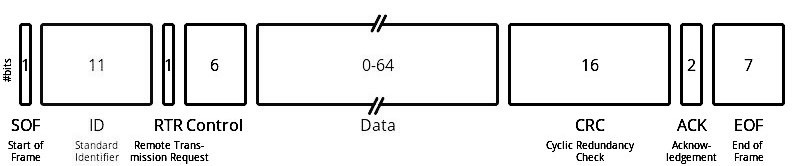
\includegraphics[scale=0.5]{immagini/CAN-bus-frame-standard-message-SOF-ID-RTR-Control-Data-CRC-ACK-EOF}\caption{Frame CAN standard}
\end{figure}

\cite{2020}

\begin{comment}
inserire immagine frame can e bibliografia
\end{comment}
\newpage{}

\section{CANopen over CAN}

Mentre CAN rappresenta i due livelli pi� bassi del modello OSI, CANopen
occupa il livello pi� alto, quello di applicazione (CiA 402\cite{Cia2002}). 

\begin{figure}[H]
\begin{centering}
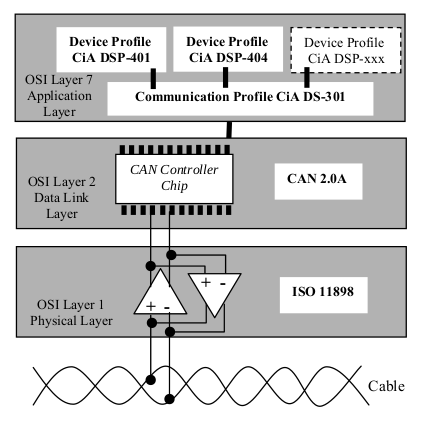
\includegraphics[scale=0.5]{immagini/CANopen-and-CAN-schematic}\caption{Schema degli standard CAN e CANopen nel modello OSI}
\cite{Boterenbrood2005}
\par\end{centering}
\end{figure}

CANopen integra al suo interno diversi concetti: 

\subsection{Object dictionary}

Ogni nodo della reta CANopen deve essere provvisto dell'object dictionary
(OD): una struttura standardizzata che contiene tutti i parametri
e i registri che descrivono il suo comportamento, dal nome del device(un
parametro statico), fino ad arrivare al target di velocit� nel caso
di un drive per motori (contenuto in un registro che deve poter essere
modificato durante il funzionamento). Ad ogni voce dell'OD si accede
tramite un indice esadecimale, a cui � aggiunto un sotto-indice a
8 bit. Per esempio per accedere alla voce che contiene la frequenza
dell'heartbeat (un parametro che ci serve per capire se il nodo sta
funzionando correttamente) utilizzeremo l'indice 0x1017, subindex
0. 

Tra i registri del drive, quelli pi� importanti nella nostra applicazione
sono ControlWord (0x6040), StatusWord (0x6041), Heartbeat (0x1017)
e Target Velocity (0x800D)\cite{Boterenbrood2005,Microphase2003,Microphase2017}. 

\begin{comment}
inserire indirizzi e citazione
\end{comment}


\subsection{Protocolli di comunicazione, SDO}

Per modificare e leggere le voci dell'object dictionary si utilizza
l'SDO, Service Data Object. L'SDO � un protocollo di comunicazione
relativamente lento in quanto ha un comportamento \textquotedbl{}client-server\textquotedbl{}
che comporta un overhead sostanziale, non � possibile utilizzarlo
per trasmettere dati in real-time. Nel nostro caso il computer di
bordo (client) inizia una comunicazione con il drive (server) e pu�
richiedere una lettura di una voce dell'OD (SDO upload) oppure pu�
modificare una voce dell'OD (SDO download). 

Ogni CAN frame di un SDO pu� portare fino a 4 byte, e ad ogni richiesta
segue una risposta. Quindi per leggere 4 byte di informazione ho bisogno
di un CAN frame per inviare la richiesta, e uno per ricevere la risposta. 

Gli SDO sono molto flessibili: permettono il trasporto di una grande
quantit� di dati utilizzando pi� CAN frames, e funzionano anche con
un nodo in modalit� pre-operational. 

Per questo motivo solitamente vengono utilizzati per il setup iniziale
di un nodo. \cite{Boterenbrood2005,Electronics2020}

\subsection{Protocolli di comunicazione, PDO}

Il PDO invece � un servizio a basso overhead (solo 4 byte) molto pi�
veloce dell'SDO, viene utilizzato per trasmettere dati in real-time.
Mentre per trasportare 8 byte di dati ad un PDO basta un CAN frame,
per trasportare la stessa informazione ad un SDO ne servirebbero 4
(due richieste e due risposte da 4 byte ciascuna). Per questo motivo
si usano i PDO per trasmettere feedback di posizione oppure per settare
un target di velocit�. \cite{Electronics2020,Boterenbrood2005}

\subsection{Profili di Moto, CiA 402}

Il CiA 402 � un profilo standardizzato per drives elettrici che implementa
diverse modalit� di funzionamento, tra cui Homing, Profile Position,
Interpolated Position, Profile Torque e Velocity. Tutte queste modalit�
sono supportate dal drive Microphase, ma quella di nostro interesse
� la modalit� a target di velocit�. 

Lo standard CiA 402 inoltre implementa una macchina a stati, che implementa
l'attivazione e il blocco del drive oltre ad altri comandi specifici
della modalit� di funzionamento impostata. \cite{Cia2002}



\chapter{Architettura e componenti Software}

\primalettera{P}er permettere al computer di bordo di inviare comandi
al drive e ricevere un feedback, � necessario trovare un modo di codificare
i messaggi ROS in CANframes.

Bench� la comunicazione non sia ancora possibile, in questo capitolo
si elencheranno i passaggi necessari ad eseguire il setup del drive,
dell'ambiente ROS, delle librerie e strumenti aggiuntivi necessari. 

\subsection{Setup drive }

I parametri statici che definiscono il funzionamento del drive devono
essere programmati attraverso una connessione seriale rs422, possibile
attraverso il convertitore moxa.

Per eseguire il setup del drive � stato necessario utilizzare Drive
Watcher, un software proprietario fornito dal produttore dei motori,
questa suite sfortunatamente � compatibile solo con windows xp e necessita
si un port non disponibile in una virtual machine il che rende impossibile
utilizzarla senza avere il sistema operativo installato. � stato quindi
necessario utilizzare una vecchio computer esclusivamente per programmare
i parametri del drive. 

\subsubsection{Abilitare Moxa}

Per abilitare il convertitore moxa � necessario per prima cosa installare
il driver da CD o file .zip della Moxa, il programma � presente all\textquoteright interno
della cartella riferita al convertitore Moxa che si possiede. Bisogna
entrare nella cartella Software, e installare file .exe. 

Per abilitare il port � necessario andare in Pannello di controllo
> Sistema > Hardware > Gestione Periferiche.
\begin{enumerate}
\item \begin{flushleft}
Da Porte (COM e LPT) cliccare col tasto destro su MOXA USB e aprire
Propriet�; in Port Settings impostare i seguenti valori : Baud Rate
= 9600, Data its = 8, Parity = None, Stop bits = 1, Flowcontrol =
None.
\begin{figure}[H]
\centering{}\includegraphics[scale=0.5]{\string"immagini/installazione moxa1\string".png}\caption{Installazione moxa, parte 1}
\end{figure}
\pagebreak{}
\par\end{flushleft}
\item \begin{flushleft}
Da Schede Seriali Multiport cliccare col tasto destro su Uport 1130I
e aprire Propriet�; in Ports Configuration aprire Port Setting della
COM in uso dalla Moxa e impostare : Fast Flush su Enable e Interface
su RS-422.
\begin{figure}[H]

\begin{centering}
\includegraphics[scale=0.5]{\string"immagini/installazione moxa2\string".png}\caption{Installazione moxa, parte2}
\par\end{centering}
\end{figure}
\par\end{flushleft}
\end{enumerate}

\subsection{Installazione Drive Watcher}

Per installare il software basta semplicemente estrarre e aprire il
file Setup-DriveWatcher-407.exe. 

Prima di modificare i parametri bisogna accertarsi che la moxa sia
connessa al driver e che la parte logica del driver sia alimentata
a 24V, con l'uscita negativa dell'alimentatore messa a terra. 

Si esegue un settaggio della comunicazione attraverso la modalit�
\textquotedbl{}Communication Settings\textquotedbl{}, impostando la
ComPort designata in precedenza e cercando il nodo attivo attraverso
il \textquotedbl{}search node tool\textquotedbl{}. L'ultimo tool menzionato
eseguir� uno sweep completo di tutti i nodi disponibili, indicando
quelli attivi con un colore differente. 

\begin{figure}[H]
\begin{centering}
\includegraphics[scale=0.5]{\string"immagini/node sweep\string".png}\caption{Communication Settings e Search Node Tool}
\par\end{centering}
\end{figure}

Una volta impostato il nodo si controlla che la connessione sia attiva
attraverso il tool \textquotedbl{}ComPort communication test\textquotedbl{}
(icona a cacciavite). 

\subsection{Programmazione dei parametri}

I parametri si possono visualizzare nella sezione \textquotedbl{}Parameters
configuration\textquotedbl{}, ogni parametro dispone di una descrizione
a lato, quindi in questo documento non si elencheranno tutti, ma solo
i pi� importanti ai fini del progetto. Per farsi un'idea pi� dettagliata
si possono consultare il manuale Siboni \textquotedbl{}Istruzioni
Drive Watcher\textquotedbl{} \cite{Siboni2018} e quello completo
del drive Microphase \textquotedbl{}Micro Digital One\textquotedbl{},
capitolo 9. \cite{Microphase}

\begin{figure}[H]

\begin{centering}
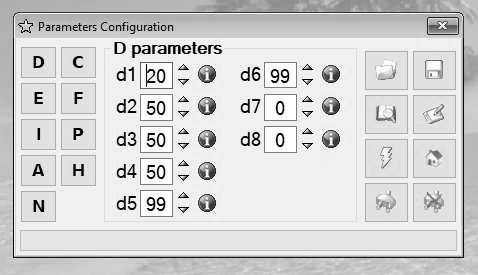
\includegraphics[scale=0.5]{immagini/parametri}\caption{lo strumento Parameters Configuration}
\par\end{centering}
\end{figure}
Fare particolare attenzione ai parametri: 
\begin{description}
\item [{C7}] numero nodo = 1 di default
\item [{C9}] modo di funzionamento del drive, impostato a 5 per il CANopen
\item [{D8}] selezione del motore utilizzato, nel nostro caso brushless
sinusoidale
\item [{N1}] bitrate CAN, impostiamo a 5 per 250Kbaud, 6 per 500Kbaud
\end{description}

\section{Setup ROS}

L'installazione di ROS varia in base alle release. In questo progetto
� stata utilizzata Melodic Morenia, ma in base alla distro di linux
installata sul computer di bordo potrebbe essere necessario installare
una release differente. Ritenendo inutile descrivere il processo di
installazione di una singola versione quando � disponibile online
ampia documentazione a riguardo, si include qui il link al sito ufficiale
di ROS, dove sono indicati tutti gli step necessari per le varie piattaforme:
\url{https://wiki.ros.org/ROS/Installation}.

Successivamente, si utilizza Catkin per creare un workspace in cui
sviluppare il progetto:

\begin{lstlisting}
$ mkdir -p ~/catkin_ws/src 
$ cd ~/catkin_ws/ 
$ catkin_make
\end{lstlisting}

Per rendere utilizzabili con roscd e roslaunch i pacchetti aggiuntivi
che installeremo nel workspace, � necessario aggiungere all'origine
il nuovo file setup.{*}sh

Dall'interno della cartella catkin\_ws, si scrive nel terminale:

\begin{lstlisting}
$ source devel/setup.bash
$ echo $ROS_PACKAGE_PATH /home/youruser/catkin_ws/src:/opt/ros/kinetic/share
\end{lstlisting}

Questo comando, insieme a catkin\_make, andr� ripetuto per sicurezza
ad ogni utilizzo del workspace e soprattuto dopo l'installazione di
nuovi pacchetti. 

\section{Setup PCAN}

Bench� dei driver per adattatore PCAN siano installati di default
nel kernel linux, per cui i canali CAN sono gestiti come dispositivi
netdev, per utilizzare il software di visualizzazione pcan\_view e
l'API pcan\_basic � necessario installare i driver proprietari. 

I driver sono disponibili sul sito della PEAK system all'indirizzo
\url{https://www.peak-system.com/fileadmin/media/linux/files/peak-linux-driver-8.10.2.tar.gz}.

Per installarli basta decomprimere il file, aprire la cartella su
un terminale e utilizzare i seguenti comandi: 

\begin{lstlisting}
$ make clear
$ sudo make
$ sudo make install
\end{lstlisting}




\chapter*{Conclusioni\aggiungiAIndice{Conclusioni}}

\primalettera{I}l cloud computing � .............

%add to index with the right hyperlink
\cleardoublepage \phantomsection \addcontentsline{toc}{chapter}{Bibliografia}\bibliographystyle{alpha}
\phantomsection\addcontentsline{toc}{chapter}{\bibname}\bibliography{bibliografia}


\chapter*{Ringraziamenti}

Grazie a Andrea che ha pubblicato il modello, anche se il grosso del
lavoro era gi� fatto da Filippo Zangheri!

\end{mainmatter}
\end{document}
